\section{Nearest neighbours}
\subsection{Classical nearest neighbours}
Figure~\ref{fig:knn} shows the results of the $k$-NN algorithm in function of the number of training data-points for a different number of neighbours. We can see that the performance is very similar to radial based function support vector machines.

A first observation is that contrary to SVMs models, the performance always keeps increasing with added number of training points. This makes sense as support vector machines have a limited complexity due to their limited number of coefficients to be trained in their primal form. This is not totally true for SMVs using kernel functions and being evaluated in the dual, but their complexity is based on the number of support vectors which are consisting of only data-points close to the decision boundary. Adding more training points only improves the performance when those are close to the decision boundary if we neglect the smoothening of the boundary --- which in our case appears not to be very important. In $k$-NN algorithm, all data-points participate to the decision boundary. Increasing the density of data-points allows the decision boundary to be influenced by any new data-point. The need for intricate boundaries --- or high complexity --- is also an explanation of the good performance of $k$-NN.

To understand the high variability of Matthew's correlation coefficient, we must take a more detailed look at the individual results (table~\ref{tab:knn}, more details in appendix~\ref{app:knn}). Matthew's correlation coefficient is computed on the binary correlation matrices for each class. For the total one, the mean is taken. As already mentioned before, the big advantage of this coefficient is that it takes into account the prior probabilities of both binary classes. This has a huge influence on the U2R class --- and in a lesser manner the R2L class --- that has very few instances. The accuracy is thus very good as very few points are classified in this category as should be for the very big majority, but the classifier is not very successful for the ones that should. As discussed before, not much can be done except increasing the number of instances of these classes.

\begin{figure}[h!]
        \begin{subfigure}[b]{.97\textwidth}  
            \centering 
            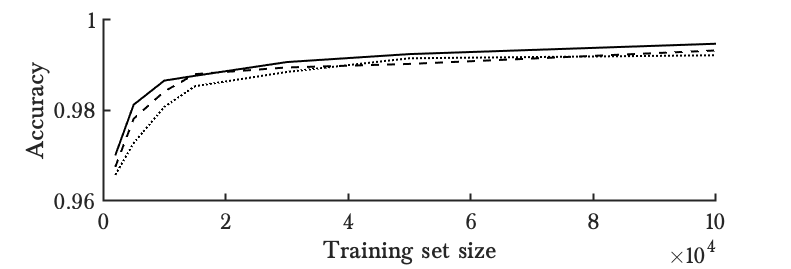
\includegraphics[width=.98\textwidth]{parts/chap-4/img-knn/knn-acc.png}
            %\caption{Accuracy in function of the number of training points for a different number of neighbours.}
        \end{subfigure}
        %\vfill
        %\begin{subfigure}[b]{.97\textwidth}  
        %    \centering 
        %    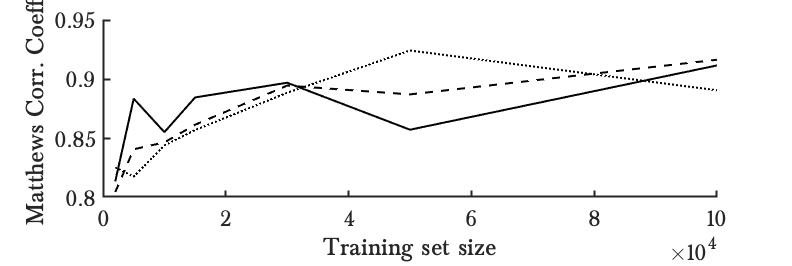
\includegraphics[width=.98\textwidth]{parts/chap-4/img-knn/knn-mcc.png}
        %    \caption{Matthew's correlation coefficient in function of the number of training points for a different number of neighbours.} 
        %\end{subfigure}
        %\vfill
        %\begin{subfigure}[b]{.97\textwidth}  
        %    \centering 
        %    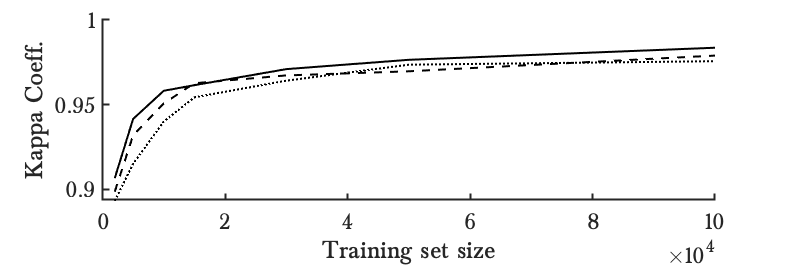
\includegraphics[width=.98\textwidth]{parts/chap-4/img-knn/knn-kappa.png}
        %   \caption{Cohen's kappa coefficient in function of the number of training points for a different number of neighbours.} 
        %\end{subfigure}
        %\vfill
        \caption[Results of $k$-NN.]{Performance of the $k$-NN algorithm in function of the number of training data-points for a different number of neighbours. The plain line is for $k=1$, the dashed is $k=2$ and the dotted is $k=3$.}
        \label{fig:knn}
\end{figure}

\begin{table}[h!]
    \centering
    \begin{tabularx}{\textwidth}{lXXXXXXXX}
    \hlineI
    Model &&& Normal & Probe & DoS & R2L & U2R & Total \\ \hlineI
    \multicolumn{9}{l}{$k=1$ with $n=10,000$}\\
    Accuracy [\%] &&& 98.17 & 99.45 & 98.80 & 98.03 & 43.33 & 98.66\\ 
    MCC [\%] &&& 97.49 & 99.19 & 98.63 & 92.76 & 39.68 & 85.55\\ 
    Kappa [\%] &&& 23.48 & 41.80 & 42.04 & 94.07 & 99.74 & 95.81\\    \hline
    Obs. Normal  &&& 2945 & 11 & 15 & 25 & 4 & \\ 
    Obs. Probe  &&& 10 & 2246 & 2 & 1 & 0 & \\ 
    Obs. DoS  &&& 23 & 3 & 2231 & 1 & 1 & \\ 
    Obs. R2L  &&& 2 & 0 & 0 & 214 & 2 & \\ 
    Obs. U2R  &&& 3 & 0 & 0 & 2 & 4 & \\  \hlineI
    \multicolumn{9}{l}{$k=1$ with $n=100,000$}\\
    Accuracy [\%] &&& 99.56 & 99.82 & 99.63 & 93.81 & 58.33 & 99.48\\ 
    MCC [\%] &&& 99.00 & 99.73 & 99.57 & 95.39 & 62.16 & 91.17\\ 
    Kappa [\%] &&& 22.61 & 41.51 & 41.58 & 94.88 & 99.85 & 98.36\\  \hline
    Obs. Normal  &&& 2987 & 4 & 4 & 5 & 1 & \\ 
    Obs. Probe  &&& 2 & 2260 & 2 & 0 & 0 & \\ 
    Obs. DoS  &&& 8 & 0 & 2256 & 0 & 0 & \\ 
    Obs. R2L  &&& 12 & 0 & 0 & 190 & 1 & \\ 
    Obs. U2R  &&& 2 & 0 & 0 & 1 & 4 & \\   \hlineI
    \end{tabularx}
    \caption[Detailed $k$-NN results.]{Detailed results of the $k$-NN classification algorithm for $k=1$ for a small and for a large training data-set.}
    \label{tab:knn}
\end{table}

\subsection{Training set reduction}
\begin{wrapfigure}[12]{r}{0.45\textwidth}
\begin{center}
    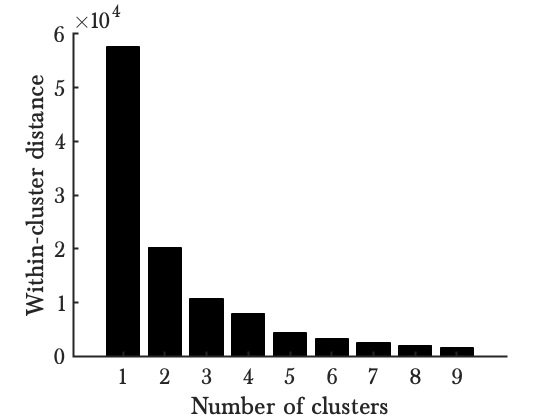
\includegraphics[width=.45\textwidth]{parts/chap-4/img-knn/kmeans.png}
    \caption{Within cluster sum of distances in function of the number of clusters chosen.}
    \label{fig:kmeans}
\end{center}
\end{wrapfigure}
The training is linearly dependent on the number of instances in the training set --- the ones that are compared to the search for the nearest neighbours. To reduce the evaluation time, we must find a way to reduce this number and the find only the relevant data-points.

\subsubsection{$k$-means clustering}
The $k$-NN does as good as the best radial based function support vector machine for $n=10,000$ instances and surpasses all the previously tested algorithms for more training points, where this is even more clear for $n=100,000$.

To select the number of clusters, the elbow rule suggests to take 5 clusters, which is by the way the same results obtained by \cite{Soheily-Khah2018IntrusionDataset}, but with a different data-set (figure~\ref{fig:kmeans}). We can then keep only the normal instances near the decision boundary, i.e. the cluster with the closest mean to the other classes. This gives very disappointing results independently of the number of nearest neighbours $k$ chosen. Table~\ref{tab:knn-kmeans} also shows the results where the sole most-distant cluster is discarded. However, the results are still very disappointing although logically better than keeping the sole best cluster, we can see that a lot of normal data-points are abusively considered as various attacks. The model lacks information about the variety of normal attacks, variety that we just suppressed. This suggests that they are no specific regions where the data-points are not relevant. In other words, the decision boundary goes through all clusters, all regions of the hyper-space where points are present. This once again confirms the complexity of the decision boundary and the problem in general. We could try to increase the number of clusters to discard smaller groups and do this iteratively always discarding the worse one, but after all, the direction this is going to is select the points individually and not based on groups. This problem is better tackled with condensed nearest neighbours.

\begin{table}[h!]
    \centering
    \begin{tabularx}{\textwidth}{lXXXXXXXX}
    \hlineI
    Model &&& Normal & Probe & DoS & R2L & U2R & Total \\ \hlineI
    \multicolumn{9}{l}{$k=1$ with $n=100,000$ and $k$-means.}\\
    Accuracy [\%] &&& 95.19 & 99.29 & 98.78 & 96.92 & 76 & 97.45\\ 
    MCC [\%] &&& 94.88 & 97.05 & 98.29 & 89.79 & 74.85 & 90.97\\ 
    Kappa [\%] &&& 25.09 & 41.02 & 41.67 & 94.85 & 99.60 & 92.02\\   \hline
    Obs. Normal  &&& 2856 & 12 & 25 & 5 & 3 & \\ 
    Obs. Probe  &&& 84 & 2251 & 2 & 0 & 0 & \\ 
    Obs. DoS  &&& 23 & 4 & 2239 & 0 & 0 & \\ 
    Obs. R2L  &&& 34 & 1 & 0 & 179 & 0 & \\ 
    Obs. U2R  &&& 4 & 0 & 0 & 0 & 11 & \\ \hlineI
    \end{tabularx}
    \caption[Comparison of the $k$-NN results.]{Detailed results of the $k$-NN classification algorithm for $k=1$ and for $n=100,000$ using $k$-means data reduction.}
    \label{tab:knn-kmeans}
\end{table}

\subsubsection{Condensed nearest neighbours}
The clustering-based methods give good results for huge data-sets and has successfully applied it to \emph{random forest classifiers}~\cite{Soheily-Khah2018IntrusionDataset}. In our case, we have a lower number of data-points and we do not try to discard the majority of them, but intelligently select the relevant ones to reduce our number of instances in the training data-set. The condensed nearest neighbours is an instance-wise selection method and not based on larger groups as are clustering methods. However, the better results of the $k=1$ does not allow us to discard the outliers.

Table~\ref{tab:knn-cnn} shows the results of the condensed nearest neighbours which appear to be almost as good as without any data reduction, but a dramatic training size decrease: from 10,000 to less than 400. This represents a data reduction of more than 96\% !

\begin{figure}[h!]
        \begin{subfigure}[b]{.97\textwidth}  
            \centering 
            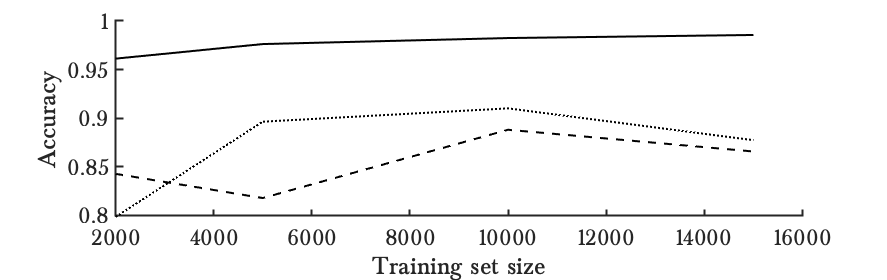
\includegraphics[width=.98\textwidth]{parts/chap-4/img-knn/cnn/acc.png}
            \caption{Accuracy with condensed nearest neighbours.}
        \end{subfigure}
        %\vfill
        %\begin{subfigure}[b]{.97\textwidth}  
        %    \centering 
        %    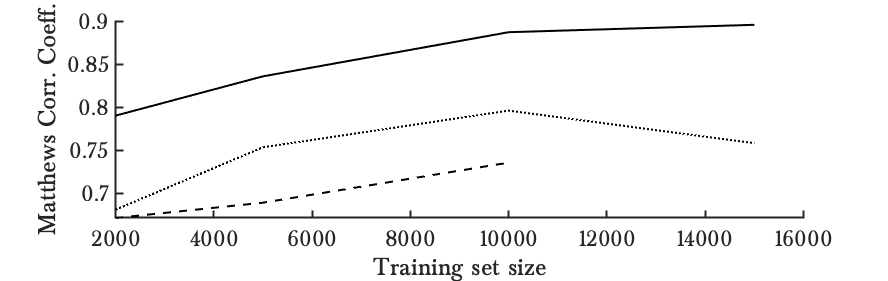
\includegraphics[width=.98\textwidth]{parts/chap-4/img-knn/cnn/mcc.png}
        %    \caption{Matthew's correlation coefficient with condensed nearest neighbours.} 
        %\end{subfigure}
        %\vfill
        %\begin{subfigure}[b]{.97\textwidth}  
        %    \centering 
        %    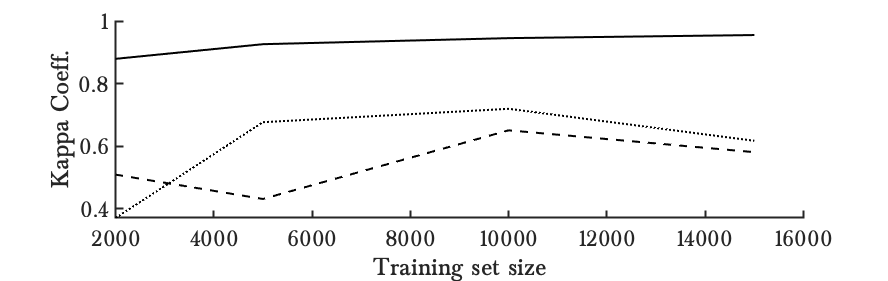
\includegraphics[width=.98\textwidth]{parts/chap-4/img-knn/cnn/kappa.png}
        %    \caption{Cohen's kappa coefficient with condensed neighbours.} 
        %\end{subfigure}
        \vfill
        \begin{subfigure}[b]{.97\textwidth}  
            \centering 
            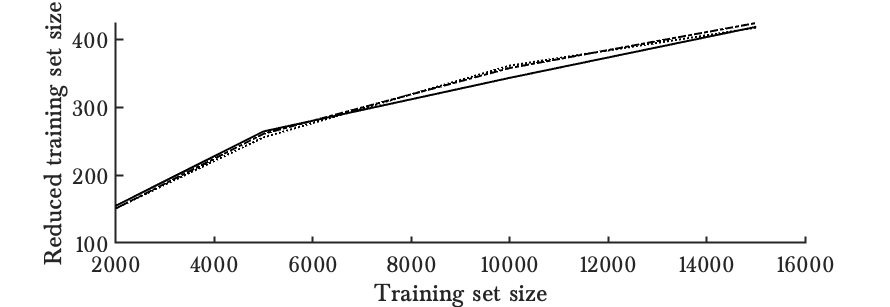
\includegraphics[width=.98\textwidth]{parts/chap-4/img-knn/cnn/red.png}
            \caption{Number of data-points after reduction.} 
        \end{subfigure}
        \caption[Comparison of the CNN results.]{Performance of the $k$-NN algorithm in function of the number of training data-points for a different number of neighbours. The plain line is for $k=1$, the dashed is $k=2$ and the dotted is $k=3$.}
        \label{fig:knn-cnn}
\end{figure}

\begin{table}[h!]
    \centering
    \begin{tabularx}{\textwidth}{lXXXXXXXX}
    \hlineI
    Model &&& Normal & Probe & DoS & R2L & U2R & Total \\ \hlineI
    \multicolumn{9}{l}{$k=1$ with $n=10,000$ and CNN.}\\
    Accuracy [\%] &&& 97.63 & 99.11 & 98.26 & 98.16 & 80 & 98.25\\ 
    MCC [\%] &&& 96.73 & 99.02 & 98.02 & 90.27 & 59.45 & 88.70\\ 
    Kappa [\%] &&& 23.74 & 41.94 & 42.19 & 93.92 & 99.70 & 94.52\\    \hline
    Obs. Normal  &&& 2929 & 14 & 31 & 3 & 1 & \\ 
    Obs. Probe  &&& 9 & 2238 & 1 & 1 & 0 & \\ 
    Obs. DoS  &&& 20 & 4 & 2219 & 0 & 0 & \\ 
    Obs. R2L  &&& 36 & 1 & 4 & 213 & 1 & \\ 
    Obs. U2R  &&& 6 & 0 & 3 & 0 & 6 & \\    \hlineI
    \end{tabularx}
    \caption[Deatiled CNN results.]{Detailed results of the $k$-NN classification algorithm for $k=1$ with condensed neighbours reduction.}
    \label{tab:knn-cnn}
\end{table}

\subsection{Feature size reduction}
The $k$-NN algorithm is composed of two phases: the computation of the distances and the searching for the smallest one. As the second phase will not be impacted by the feature size reduction, this is not the case for the computation of the distances which --- as already observed before --- increase linearly with the feature size. Of course, the computation of the PCA components has a certain cost, but it becomes marginal in comparison to the total cost as the number of distances to be computed increases. There is no additional cost for the $\chi^2$ feature reduction but it usually keeps more features.

\subsubsection{Principal components analysis}
In comparison to the support vector machines with nearest neighbors, a much lower number of principal components seems to be needed (figure~\ref{fig:knn-cnn-pca}). However, the loss of allowed complexity of the model due to the feature size reduction results in more instances to be retained after the CNN reduction. The loss of complexity is compensated by an increase of complexity in the instance dimension, this to allow complex decision boundaries. However, the difference is here relatively marginal: about 430 instances compared to 380. Let us compare the total information retained in the model: $n_t \times (n_p+1)$ where $n_t$ and $n_p$ are the instance and feature size (number of components) after reduction. The $+1$ corresponds to class associated with each instance. The case with 8 components corresponds to a total information reduction of almost 47\% compared to the case with 16 components. Though, both have pretty much the same classification performance.

\begin{figure}[h!]
        \begin{subfigure}[b]{.97\textwidth}  
            \centering 
            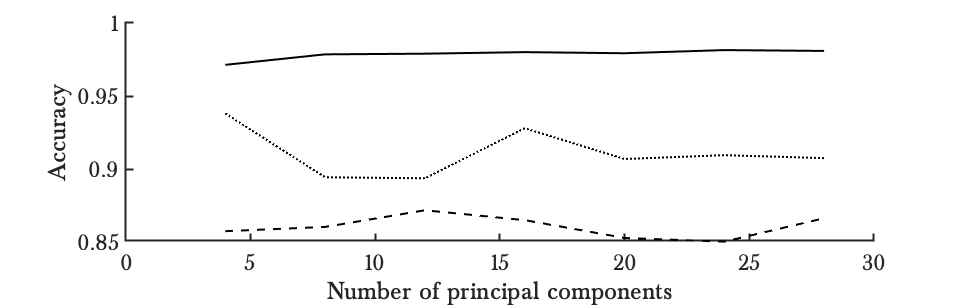
\includegraphics[width=.98\textwidth]{parts/chap-4/img-knn/cnn-pca/acc.png}
            \caption{Accuracy with condensed nearest neighbours in function of the number of PCA components.}
        \end{subfigure}
        \vfill
        \begin{subfigure}[b]{.97\textwidth}  
            \centering 
            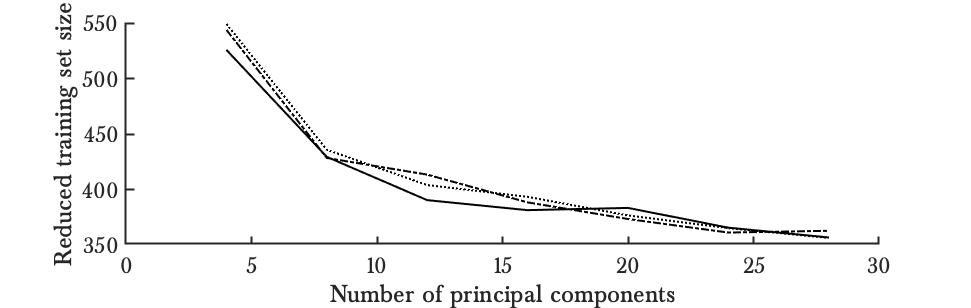
\includegraphics[width=.98\textwidth]{parts/chap-4/img-knn/cnn-pca/red.png}
            \caption{Instance set size after reduction in function of the number of PCA components.} 
        \end{subfigure}
        \caption[CNN results with PCA.]{Performance of the $k$-NN algorithm with PCA reduction and CNN reduction in function of the number of principal components retained. The plain line is for $k=1$, the dashed is $k=2$ and the dotted is $k=3$.}
        \label{fig:knn-cnn-pca}
\end{figure}

However, compared to the CNN without PCA reduction, the accuracy is slightly diminishing, but still resulting in very good results (table~\ref{tab:knn-cnn-pca}, more results in appendix~\ref{app:knn-cnn-pca}).

\begin{table}[h!]
    \centering
    \begin{tabularx}{\textwidth}{lXXXXXXXX}
    \hlineI
    Model &&& Normal & Probe & DoS & R2L & U2R & Total \\ \hlineI
    \multicolumn{9}{l}{$k=1$ with $n=10,000$, $n_{pca}=8$ and CNN.}\\
    Accuracy [\%] &&& 97.27 & 98.81 & 98.18 & 95 & 51.67 & 97.85\\ 
    MCC [\%] &&& 96.15 & 98.25 & 97.79 & 89.08 & 43.98 & 85.05\\ 
    Kappa [\%] &&& 23.90 & 41.87 & 42.13 & 94.29 & 99.63 & 93.29\\     \hline
    Obs. Normal  &&& 2918 & 16 & 32 & 7 & 5 & \\ 
    Obs. Probe  &&& 20 & 2233 & 9 & 0 & 0 & \\ 
    Obs. DoS  &&& 21 & 8 & 2219 & 0 & 0 & \\ 
    Obs. R2L  &&& 34 & 2 & 0 & 198 & 1 & \\ 
    Obs. U2R  &&& 7 & 0 & 0 & 4 & 6 & \\    \hlineI
    
    \multicolumn{9}{l}{$k=1$ with $n=10,000$, $n_{pca}=16$ and CNN.}\\
    Accuracy [\%] &&& 97.16 & 98.68 & 98.61 & 96.78 & 86.00 & 98.00\\ 
    MCC [\%] &&& 96.30 & 98.33 & 98.22 & 89.69 & 55.24 & 87.56\\ 
    Kappa [\%] &&& 24.00 & 41.91 & 41.92 & 94.30 & 99.56 & 93.77\\     \hline
    Obs. Normal  &&& 2915 & 22 & 24 & 5 & 0 & \\ 
    Obs. Probe  &&& 17 & 2232 & 7 & 0 & 0 & \\ 
    Obs. DoS  &&& 19 & 6 & 2231 & 0 & 0 & \\ 
    Obs. R2L  &&& 35 & 2 & 1 & 198 & 1 & \\ 
    Obs. U2R  &&& 14 & 0 & 0 & 1 & 9 & \\     \hlineI
    \end{tabularx}
    \caption[Detailes results of the CNN with PCA.]]{Detailed results of the $k$-NN classification algorithm for $k=1$ with condensed neighbours reduction and PCA reduction.}
    \label{tab:knn-cnn-pca}
\end{table}

\subsubsection{$\chi^2$ feature selection}
Here again, we can also use a $\chi^2$ feature selection instead of a PCA decomposition (figure~\ref{fig:knn-chi2-res} and table~\ref{tab:knn-chi2-res}). This gives a better classification performance than the original condensed nearest neighbours (table\ref{tab:knn-cnn}) for the same size training set size after reduction. The results of the relevance of each feature for each class are given at figure~\ref{fig:knn-chi2-feat} and result in similar selections as with SVMs, but the differences are more marked. Here again, we select 33 features based on the scores using the same threshold of 10 on the mean measure of each feature\footnote{The same 33 features are selected as RBF-SVMs with the same resulting p-value}. We have also tested with setting a higher threshold ($100$) of the $\chi^2$ measure and select only 20 features, but results in lower performance than the PCA reduction with $n_{pca}=16$ leading to discard this option (appendix~\ref{app:knn-cnn-chi2}).

\begin{figure}[h!]
        \begin{subfigure}[b]{.97\textwidth}  
            \centering 
            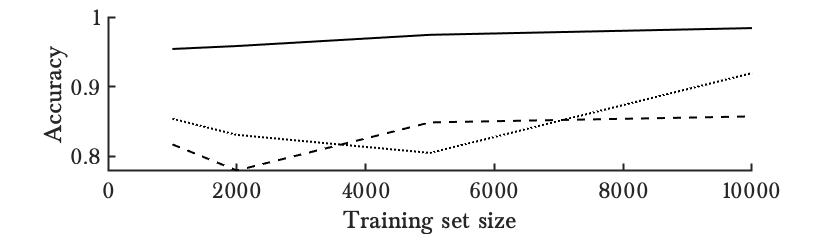
\includegraphics[width=.98\textwidth]{parts/chap-4/img-knn/cnn-chi2/acc.png}
            \caption{Accuracy with condensed nearest neighbours and $\chi^2$ feature selection.}
        \end{subfigure}
        \vfill
        \begin{subfigure}[b]{.97\textwidth}  
            \centering 
            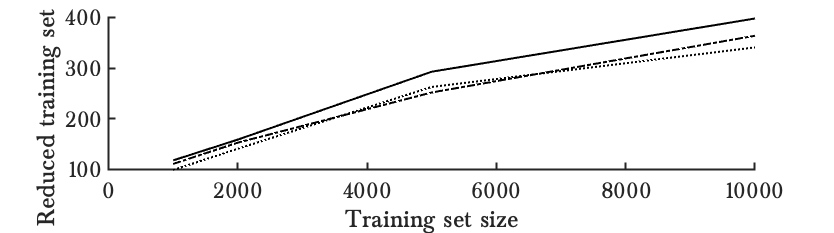
\includegraphics[width=.98\textwidth]{parts/chap-4/img-knn/cnn-chi2/red.png}
            \caption{Instance set size after reduction with condensed nearest neighbours and $\chi^2$ feature selection.} 
        \end{subfigure}
        \caption[Results of CNN with $\chi^2$ feature selection.]{Performance of the $k$-NN algorithm with $\chi^2$ feature selection (33) and CNN reduction. The plain line is for $k=1$, the dashed is $k=2$ and the dotted is $k=3$.}
        \label{fig:knn-chi2-res}
\end{figure}

\begin{table}[h!]
    \centering
    \begin{tabularx}{\textwidth}{lXXXXXXXX}
    \hlineI
    Model &&& Normal & Probe & DoS & R2L & U2R & Total \\ \hlineI
    \multicolumn{9}{l}{$k=1$ with $n=10,000$, $\chi^2$ and CNN.}\\
    Accuracy [\%] &&& 97.77 & 99.16 & 98.85 & 97.60 & 88.89 & 98.48\\ 
    MCC [\%] &&& 96.98 & 99.03 & 98.91 & 92.61 & 45.63 & 86.63\\ 
    Kappa [\%] &&& 23.66 & 41.82 & 41.97 & 94.35 & 99.44 & 95.24\\       \hline
    Obs. Normal  &&& 2933 & 15 & 24 & 5 & 0 & \\ 
    Obs. Probe  &&& 12 & 2242 & 0 & 0 & 0 & \\ 
    Obs. DoS  &&& 7 & 2 & 2235 & 0 & 0 & \\
    Obs. R2L  &&& 22 & 2 & 2 & 203 & 1 & \\ 
    Obs. U2R  &&& 26 & 0 & 0 & 0 & 8 & \\    \hlineI
    \end{tabularx}
    \caption[Deatiled results of CNN with $\chi^2$ feature selection.]{Detailed results of the $k$-NN classification algorithm for $k=1$ with condensed neighbours reduction and $\chi^2$ feature selection.}
    \label{tab:knn-chi2-res}
\end{table}

\begin{figure}[h!]
        \begin{subfigure}[b]{.87\textwidth}  
            \centering 
            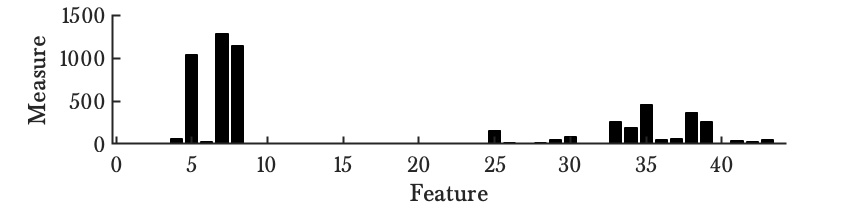
\includegraphics[width=.98\textwidth]{parts/chap-4/img-knn/cnn-chi2/normal.png}
            \caption{Normal.} 
        \end{subfigure}
        \vfill
        \begin{subfigure}[b]{.87\textwidth}  
            \centering 
            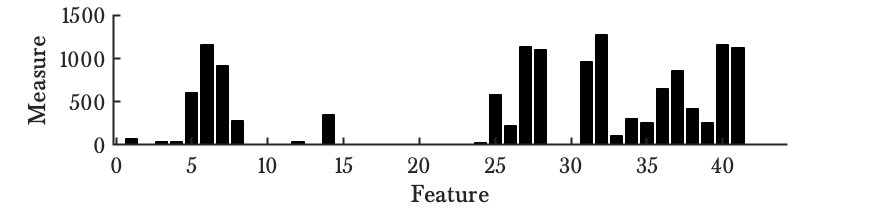
\includegraphics[width=.98\textwidth]{parts/chap-4/img-knn/cnn-chi2/dos.png}
            \caption{DoS.} 
        \end{subfigure}
        \vfill
        \begin{subfigure}[b]{.87\textwidth}  
            \centering 
            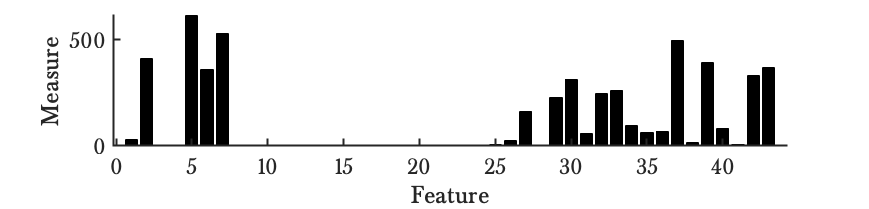
\includegraphics[width=.98\textwidth]{parts/chap-4/img-knn/cnn-chi2/probe.png}
            \caption{Probe.} 
        \end{subfigure}
        \vfill
        \begin{subfigure}[b]{.87\textwidth}  
            \centering 
            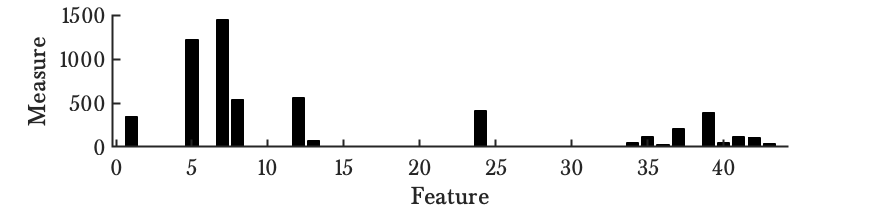
\includegraphics[width=.98\textwidth]{parts/chap-4/img-knn/cnn-chi2/r2l.png}
            \caption{R2L.} 
        \end{subfigure}
        \vfill
        \begin{subfigure}[b]{.87\textwidth}  
            \centering 
            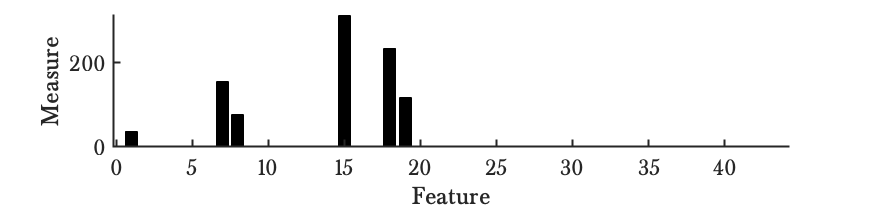
\includegraphics[width=.98\textwidth]{parts/chap-4/img-knn/cnn-chi2/u2r.png}
            \caption{U2R.} 
        \end{subfigure}
        \caption[Feature relevance using the $\chi^2$-measure with $k$-NN.]{$\chi^2$ measure of the $k$-NN algorithm for each feature and for each class.}
        \label{fig:knn-chi2-feat}
\end{figure}

\subsection{Secure evaluation}
We can now estimate the different models according to the computational cost, the round cost and the communication cost (figure~\ref{fig:eval-knn}). The accuracy is plotted here with the same value for each training set size using condensed nearest neighbours as it is not a parameter but a result of the reduction. Good performance have training set sizes after reduction ranging between approximately 300 and 500 for an original size of respectively 10,000 and 50,000. We benchmark the secure nearest neighbours algorithm with $n=200$, $n=500$ and $n=1000$. The models tested are
\begin{itemize}
    \item \textbf{(P)-1NN:} secure nearest neighbours evaluation with $k=1$;
    \item \textbf{(P)-2NN:} secure nearest neighbours evaluation with $k=2$;
    \item \textbf{(P)-3NN:} secure nearest neighbours evaluation with $k=3$;
    \item \textbf{(P)PCA8-(P)-1NN:} secure nearest neighbours evaluation with secure PCA decomposition using 8 principal components;
    \item \textbf{(P)PCA16-(P)-1NN:} secure nearest neighbours evaluation with secure PCA decomposition using 16 principal components;
    \item \textbf{$\chi^2$-(P)1NN:} secure nearest neighbours evaluation with $\chi^2$ feature selection (33).
\end{itemize}
From the previous classification performance analysis, we know that the $\chi^2$ does perform better for the same training set size after reduction. The reduction to 33 features also leads to a smaller distance evaluation which reduces the global evaluation time. The round communication costs are very similar as the largest contributor is the selection phase, which is the same. The secure nearest neighbours with $\chi^2$ feature selection is thus as good or better in all indicators than the version without and should always be preferred.

The use of PCA decomposition however leads to a very significant decrease of the run time. Indeed, the extra cost of computing the decomposition is largely compensated by the reduction of features during the distance computation. The accuracy is not as good as the previous methods, nor is it significantly worse. The secure nearest neighbours should be preferred if a very small classification performance loss is accepted in order to divide the execution time almost by half.

\begin{figure}[h!]
        \begin{subfigure}[b]{.49\textwidth}  
            \centering 
            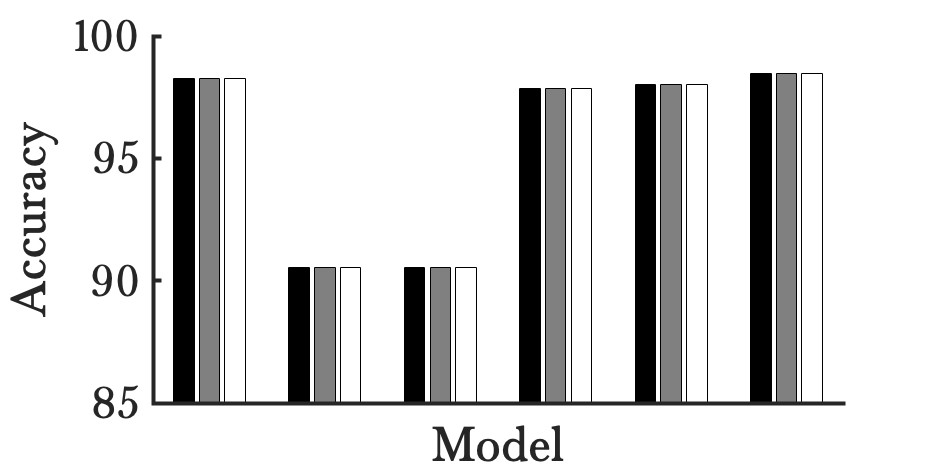
\includegraphics[width=.98\textwidth]{parts/chap-4/img-knn/knn-timing/acc.png}
            \caption{Classification performance.} 
        \end{subfigure}
        \hfill
        \begin{subfigure}[b]{.49\textwidth}   
            \centering 
            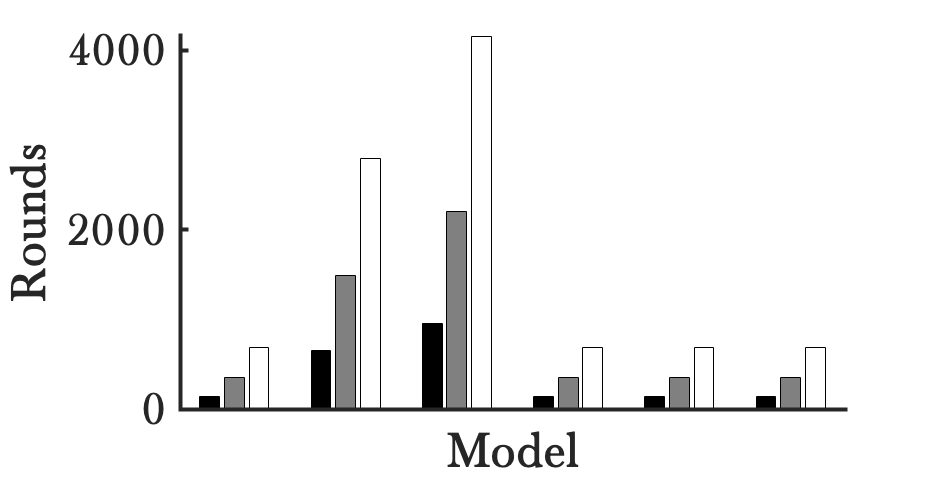
\includegraphics[width=.98\textwidth]{parts/chap-4/img-knn/knn-timing/rounds.png}
            \caption{Round cost.} 
        \end{subfigure}
        \hfill
        \begin{subfigure}[b]{.49\textwidth}   
            \centering 
            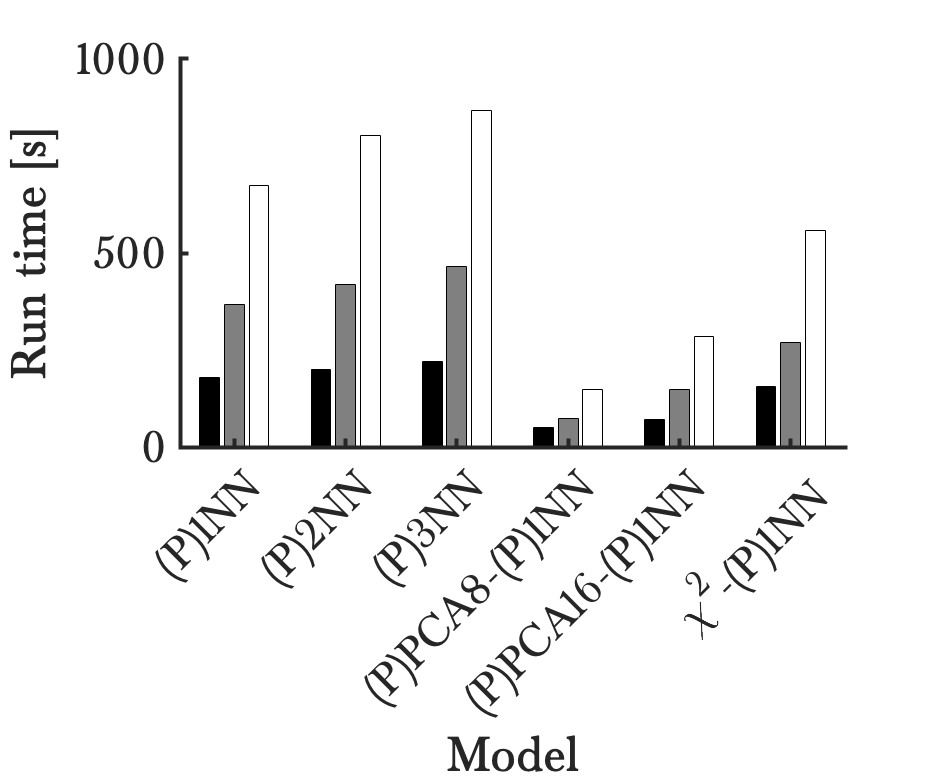
\includegraphics[width=.98\textwidth]{parts/chap-4/img-knn/knn-timing/time.png}
            \caption{Computational cost.} 
        \end{subfigure}
        \hfill
        \begin{subfigure}[b]{.49\textwidth}   
            \centering 
            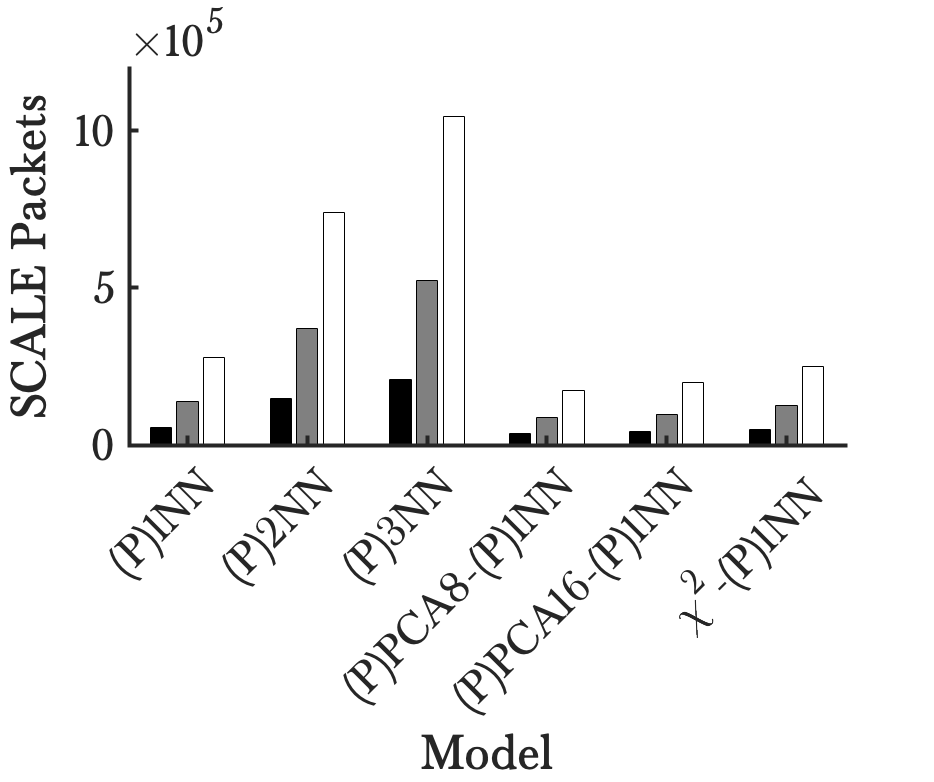
\includegraphics[width=.98\textwidth]{parts/chap-4/img-knn/knn-timing/comm.png}
            \caption{Communication cost.} 
        \end{subfigure}
        \caption[Comparison of the different $k$-NN models using MPC.]{Comparison of different protocols for secure nearest neighbours evaluation with and without various feature size reduction methods. The black bars correspond to a training set size of $n=200$, the grey to $n=500$ and the white to $n=1000$. The results correspond here to the secret evaluation of one unique query.}
        \label{fig:eval-knn}
\end{figure}

\FloatBarrier